\documentclass{article}
\usepackage[utf8]{inputenc}
\usepackage{titling}
\usepackage{graphicx}
\usepackage{xcolor}
\usepackage[colorlinks=true,linkcolor=darkgray, urlcolor =gray]{hyperref}
\usepackage[spanish]{babel}
\DeclareUnicodeCharacter{301}{~}
\usepackage{url}
\DeclareUnicodeCharacter{202F}{\,}


\title{Práctica redes Ad-hoc}
\author{Cristina Díaz García}
\date{Enero 2019}

\renewcommand\maketitlehooka{\null\mbox{}\vfill}
\renewcommand\maketitlehookd{\vfill\null}


\begin{document}

\addcontentsline{toc}{section}{Índice general}

\begin{titlingpage}
\maketitle

\begin{center}
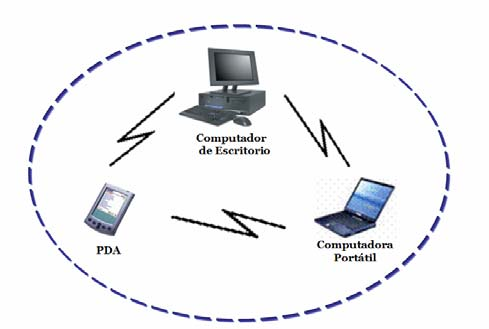
\includegraphics[scale=0.6]{adhoc.png} 
\end{center}

\end{titlingpage}

\newpage

\tableofcontents

\newpage

\section{Ejercicio 1. Estudio del algoritmo AODV con Dynamic Ad Hoc Routing Simulator (DARS)}

Creamos la topología y la simulamos:

\begin{center}
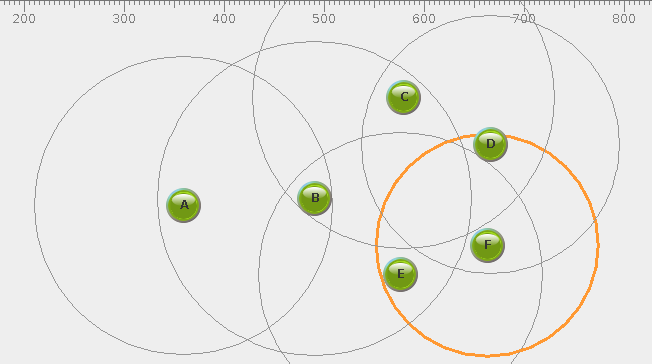
\includegraphics[scale=0.4]{sc.png} 
\end{center}

\textbf{6. Envía un mensaje de A a D (haciendo click derecho en A). En la pantalla observa la
secuencia de eventos que suceden (mensajes intercambiados, log, actualización de la
tabla de encaminamiento de los nodos, etc.). ¿Es posible el envío del mensaje? ¿Qué
ruta siguen los mensajes?}

\begin{center}
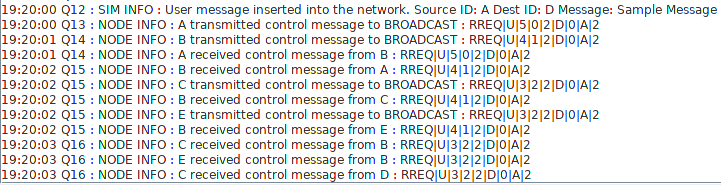
\includegraphics[scale=0.5]{log1.png}
\end{center}

\begin{center}
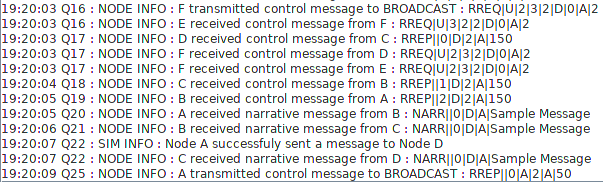
\includegraphics[scale=0.5]{log2.png}
\end{center}

Lo es, sigue el camino A-B-C-D.\\
                                                                                                                                                                                                                                                                                                                                                                                                                                                                                                                                                                                                                                                    
\textbf{7. ¿Qué nodo(s) envía(n) un RREQ? ¿Cuál es la función de este mensaje?}                                                                                                                                                                                                                                                                                                                                                                                                                                                                                                                                                                                                                                                    

A, B, C, E. Busca la ruta desde el nodo origen hasta el nodo destino.\\

\textbf{8. ¿Qué nodo(s) envía(n) un RREP? ¿Cuál es la función de este mensaje?}

D, C y B. Envía la ruta desde el nodo destino hasta el origen.\\

\textbf{9. Inmediatamente después del intento de enviar el mensaje (representado con un flujo
de mensajes en negro entre los nodos en el simulador), pausa la simulación y echa un
vistazo a la tabla de encaminamiento (vectores distancia en caché) del nodo B. ¿Qué
significa cada entrada en la tabla?}

\begin{center}
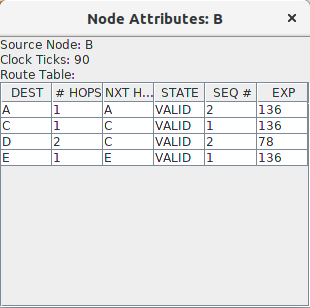
\includegraphics[scale=0.5]{nodob.png}
\end{center}

Por orden de izquierda a derecha, el destino, el número de saltos, el siguiente nodo al que saltar, el estado del enlace, la "frescura" de la ruta (el tiempo que hace que no se actualiza) y el tiempo de vida que tiene el enlace.\\

\textbf{10. Fíjate en el campo EXP de esa tabla de encaminamiento. Sin cerrar esa ventana,
reanuda la simulación (y acelera la velocidad si es necesario). ¿Qué ocurre con esos
valores? Verás que tras cierto tiempo, las entradas de la tabla cambian. Según el funcionamiento del algoritmo AODV que hemos visto en clase, ¿cómo se explica este
suceso?}

\begin{center}
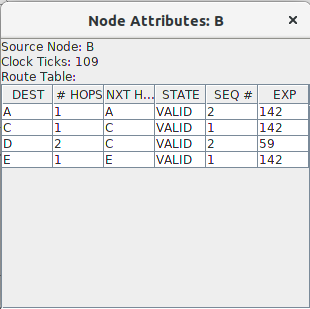
\includegraphics[scale=0.5]{nodeb2.png}
\end{center}

Porque los nodos envían mensajes periódicos para confirmar o acualizar los enlaces.\\

\textbf{11. Elimina el nodo C y a continuación envía el mismo mensaje desde A hasta D. ¿Cuál es el resultado de aplicar ahora el algoritmo de encaminamiento?}

\begin{center}
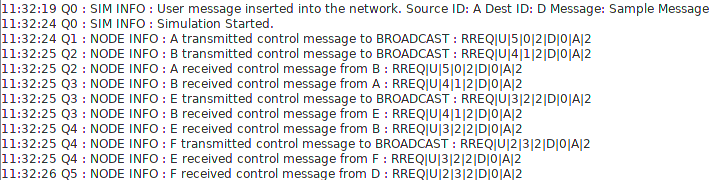
\includegraphics[scale=0.5]{log3.png}
\end{center}

\begin{center}
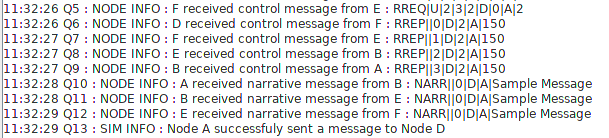
\includegraphics[scale=0.5]{log4.png}
\end{center}

El camino nuevo es A-B-E-F-D.\\

\textbf{12. Justo tras enviar el mensaje anterior pausa la simulación y, con ella pausada, encarga un envío de un mensaje con el mismo emisor y destinatario, para cuando la
simulación se reanude. No obstante, antes de reanudar la simulación (con objeto de
que la caché de los nodos sea aún válida), aleja el nodo F lo suficiente para que no
esté en el rango de los demás nodos. Ahora sí, reanuda la simulación. ¿Qué tipo de mensaje se genera para notificar ante este cambio inesperado en la ruta? ¿Quién genera este mensaje para avisar al emisor? ¿Es posible efectuar el envío? Apóyate en el log del programa si es necesario.}

\begin{center}
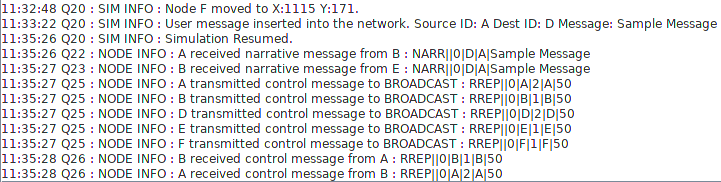
\includegraphics[scale=0.5]{log5.png}
\end{center}

\begin{center}
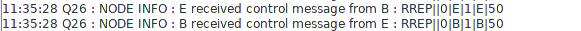
\includegraphics[scale=0.5]{log6.png}
\end{center}

Se generan \textit{Narrative messages} tanto desde B como desde E, ya que son los nodos intermedios en la ruta. Al no haber conexión con D, no se puede enviar el mensaje.
                                                                                                                                                                                                                                                                                                                                                                                                                                                                                                                                                                                                                                                     \section{Ejercicio 2. Investigación sobre otros algoritmos de encaminamiento}
                                                                                                                                                                                                                                                                                                                                                                                                                                                                                                                                                                                                                                                     
                                                                                                                                                                                                                                                                                                                                                                                                                                                                                                                                                                                                                                                  El algoritmo estudiado es WRP (Wireless Routing Protocol), una versión mejorada del protocolo de enrutamiento por vector de distancia, que usa el algoritmo de Bellman-Ford para calcular las rutas.
                                                                                                                                                                                                                                                                                                                                                                                                                                                                                                                                                                                                                                                  \\                                                                                                                                                                                                                                                                                                                                                                                                                                                                                                                                                                                                                                        	Ya que los nodos en redes MANET son móviles, el protocolo reduce los bucles de ruta y aseguran la fiabilidad del intercambio de mensajes a traves de varios mecanismos.
\\
	Para contrarrestar el problema de la cuenta hasta el infinito y para permitir una convergencia más rápida, emplea un método único para mantener la información sobre la distancia más corta a cada nodo de destino en la red y el penúltimo salto en la ruta a cada nodo de destino. WRP, al igual que DSDV, mantiene una vista actualizada de la red, cada nodo tiene una ruta fácilmente disponible para cada nodo de destino en la red. Se diferencia de DSDV en el mantenimiento de tablas y en los procedimientos de actualización: mientras que DSDV mantiene solo una tabla de topología, WRP usa un conjunto de tablas para mantener información más precisa. Las tablas que mantiene un nodo son las siguientes: tabla de distancia (DT), tabla de enrutamiento (RT), tabla de coste de enlace (LCT) y una lista de retransmisión de mensajes (MRL).
\\
	La tabla de distancia (DT) contiene la vista de red de los vecinos de un nodo, una matriz donde cada elemento contiene la distancia y el penúltimo nodo informado por un vecino para un destino en particular. La tabla de enrutamiento (RT) contiene la vista actualizada de la red para todos los destinos conocidos, mantiene la distancia más corta, el penúltimo predecesor, el nodo sucesor (el siguiente nodo que llega al destino) y una bandera que indica el estado de la ruta. El estado de la ruta puede ser una ruta simple, un bucle (error) o el nodo de destino no marcado (nulo). La tabla de coste de enlace (LCT) contiene el coste de retransmitir mensajes a través de cada enlace, siendo el coste de un enlace roto infinito. También contiene la cantidad de intervalos entre dos actualizaciones periódicas sucesivas que se han pasado desde que se recibió la última actualización exitosa desde ese enlace. Esto se hace para detectar roturas de enlaces. La lista de retransmisión de mensajes (MRL) contiene una entrada para cada mensaje de actualización que debe retransmitirse y mantiene un contador para cada entrada. Este contador disminuye después de cada retransmisión de mensaje de actualización. Cada mensaje de actualización contiene una lista de actualizaciones. Los nodos también marcan cada nodo en la RT que tiene que reconocer el mensaje de actualización que transmitió. Una vez que el contador llega a cero, las entradas en el mensaje de actualización para las cuales no se han recibido ACKs se retransmitirán y el mensaje de actualización se eliminará. Por lo tanto, un nodo detecta una ruptura de enlace por el número de periodos de actualización perdidos desde la última transmisión exitosa. Tras recibir un mensaje de actualización, los nodos no solo actualizan la distancia para los vecinos de transmisión, sino que también verifican la distancia de los otros vecinos, por lo que la convergencia es mucho más rápida que la DSDV.                                                                                                                                                                                                                                                                                                                                                                                                                                                                                                                                                                                                                                                
                                                                                                                                                                                                                                                                                                                                                                                                                                                                                                                                                                                                                                               
\end{document}